\qs{}{
    How many students are enrolled per subject?
}

Create a `VIEW` to `COUNT` the number of enrolled students for each unique course. Use `SUM` to add the total number of enrolled students per unique course, including different course versions.
\vspace{\baselineskip}

\sol{}
\noindent\line(1, 0){0.89\linewidth}
\begin{verbatim}
CREATE VIEW stude_per_course AS
SELECT c.crs_code, c.crs_name, COUNT(DISTINCT s.stud_id) AS enrolled_students_count
FROM course c
LEFT JOIN student s ON c.crs_id = s.crs_id
GROUP BY c.crs_code, c.crs_name;

SELECT stu.crs_code, stu.crs_name, SUM(stu.enrolled_students_count) AS total_enrolled_students_count
FROM stu_per_course stu
GROUP BY stu.crs_code, stu.crs_name;
\end{verbatim}
\noindent\line(1, 0){\linewidth}

\begin{figure}[H]
    \centering
    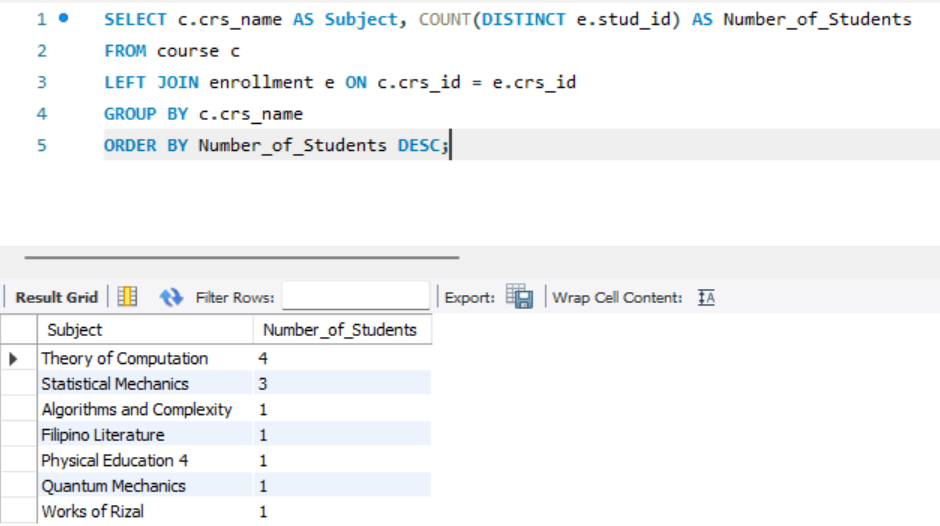
\includegraphics[width=0.7\linewidth]{images/q3.png}
    \caption{Question 3 Query and Output}
\end{figure}
